\chapter{Implementación de datos estructurados}

\section{QA como interfaz a una DB}
\subsection{Integración en sistemas open domain}
\section{Sistema}

\subsection{Corpus inicial}

\subsubsection{Grafo Mitic}
Los datos originales del proyecto mitic constan de una serie de documentos 
xml y de cinco colecciones de mongodb y relaciones entre ellas (una base de datos no relacional).

Las cinco coleccciones son: universidades, investigadores, empresas,
publicaciones, proyectos y temáticas.

Estas colecciones definen el dominio. Cada entidad 
posee sus respectivos atributos y distintas relaciones con otras entidades.
Estas relaciones contienen desde vínculos explicitos como "trabajar-en"
pero también relaciones inferidas mediante distintos algoritmos durante el proyecto mitic.
Las relaciones que incorporamos tienen distintos pesos según este tipo de caracteristicas
y tejen un grafo de distancias más o menos "especulativas" entre todas las entidades.

Los atributos de cada entidad se pueden ver en el Anexo: [[HACER Y LINKEAR]].

\subsection{Creación de Indices}

\begin{figure}[H]
  \centering
    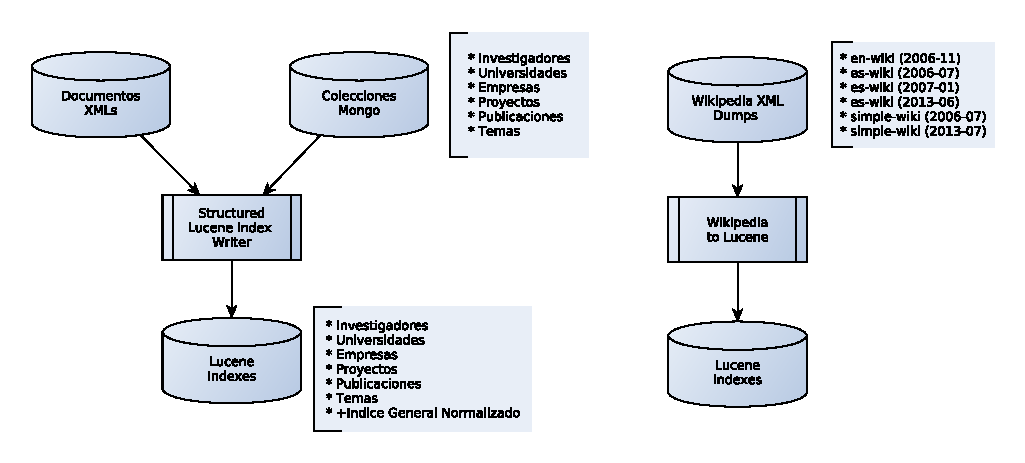
\includegraphics[scale=0.86]{graficos/LuceneWritersJuntos}
  \caption{Creación de Indices}
  \label{fig:LuceneIndexWriterBoth}
\end{figure}

A partir de esta base de datos de mongo y de los archivos xml fueron construidos cinco índices
de búsqueda lucene y un índice de búsqueda más, general, con la
información normalizada de los otros cinco. 
Cada uno de los cinco índices por entidad mantiene la estructura del tipo como campos de los documentos.
Esto quiere decir que el índice invertido para \emph{Investigadores} tiene los mismos campos
del modelo de datos de nosql. Además, se agregó el campo ``all" que resulta de la concatenación de
todos los campos. Este campo resulta útil a la hora de filtrar resultados. 
El índice general posee un documento por cada entidad de las cinco colecciones, 
manteniendo también un puntero a la entidad original y su tipo.
%El proceso de creación de índices se ilustra en la Figura \ref{fig:LuceneIndexWriterEstructurado}%~\nameref{fig:LuceneIndexWriterEstructurado}.

% \begin{figure}[H]
%   \centering
%     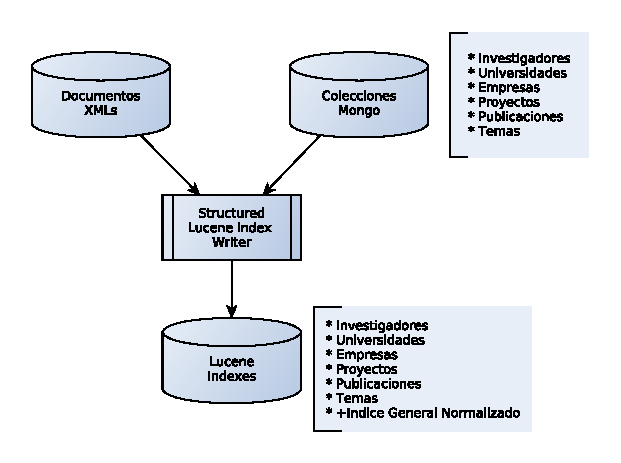
\includegraphics{graficos/LuceneIndexWriterEstructurado}
%   \caption{Lucene Index Writer para datos del proyecto Mitic}
%   \label{fig:LuceneIndexWriterEstructurado}
% \end{figure}



\subsection{Interfaz de servicios}
\label{subsec:modelos-db}
La creación offline de índices lucene tiene como finalidad optimizar
la base de conocimiento para responder con mayor eficiencia 
a búsquedas de resultados en un momento posterior. 

En esta sección vamos a ver la interfaz que presenta la base de conocimientos indexada 
al resto de los módulos del sistema y qué dependencias existen con los módulos de
análisis lingüístico.

Para la base de conocimiento estructurada, reutilizamos un modelo de datos
escrito en java  del grafo de entidades que obtuvimos de los investigadores del proyecto mitic (Ver \allref{sec:modelos-morphia}).
A estos modelos se les agregó soporte para su representación como documento dentro de un índice.
Por ejemplo, el modelo para la entidad ``Universidad de Buenos Aires", además de
persistirse en la colección de universidades de la base de datos de mongo, también dispone de una representación como documento en 
un índice lucene particular (el índice de universidades) y otra en el índice general.
A nivel colecciones, cada entidad dispone de un representante que maneja el acceso a su colección en la base de datos y también a su índice. A partir de estos representantes por entidad que ofrecen acceso a una base de datos y a un índice creamos la interfaz \emph{KnowlegdeBase}. 
Cada entidad tiene una interfaz de administración de sus dos motores de persistencia. Las responsabilidades de esta interfaz son las de un handler de conocimiento acerca de una cierta clase de entidades. 
Además, esta interfaz permite la reificación de entidades implicitas en el modelo. Estas entidades son: Ciudad, Provincia, Centro de Investigación, etc \footnote{hacer y escribir bien}. Esta reificación significa abstraer las funciones directas contra la base de datos. Mientras el $KnowledgeBase$ de Investigadores habla directo contra la base mongo o contra lucene, el $KnowlegdeBase$ de Ciudades habla contra Investigadores, Universidades y Empresas verificando ciertos campos y recomponiendo la forma de la entidad, de modo abstracto y sin persistencia propia. 

[[Tablita con totales por entidad]]

\bigskip

[[Relaciones solo presentes en mongo]]

\bigskip

Las $KnowledgeBase$ de las cinco entidad y el índice general están, a su vez, controlados un $KnowlegdeManager$, que es la interfaz del módulo que maneja la base de conocimiento. 

El $KnowledgeManager$ ofrece diferentes servicios de verificación de entidades. Para una cadena de tokens cualquiera, este módulo puede decidir, con un cierto grado de confianza, los siguientes problemas:

\begin{itemize}
  \item Si la cadena de tokens es una entidad dentro del modelo de datos. Esto incluye:
    \begin{itemize}
      \item Es una entidad del modelo de datos: una universidad, una empresa, un investigador, un proyecto, una publicacion o una tematica
      \item Es una entidad inferida: una ciudad, una provincia, un centro de investigación, un lugar de trabajo
    \end{itemize}
  \item Si la cadena es una colección del modelo de datos, es decir, si se están nombrando \dblquote{Investigadores} o \dblquote{Universidades} como clase de entidades.
  \item Si la cadena es un atributo o una relación de una clase de entidades.
\end{itemize}

La primer verificación utiliza campos de identidad de las entidades y diferentes tipos de comparadores (Ver apéndice \allref{sec:comparadores} ). Cada entidad fue configurada con diferentes atributos de identidad y a su vez estos atributos están asociados a diferentes comparadores a con un cierto grado de peso y de confianza en el juicio general. 

La segunda y la tercera verificación utiliza estos mismos comparadores jerarquizados, pero compara las cadenas de entrada contra diccionario de sinónimos escrito a mano nombrando las diferentes clases de entidades y los atributos de cada una de ellas. 

\begin{figure}[H]
  \centering
    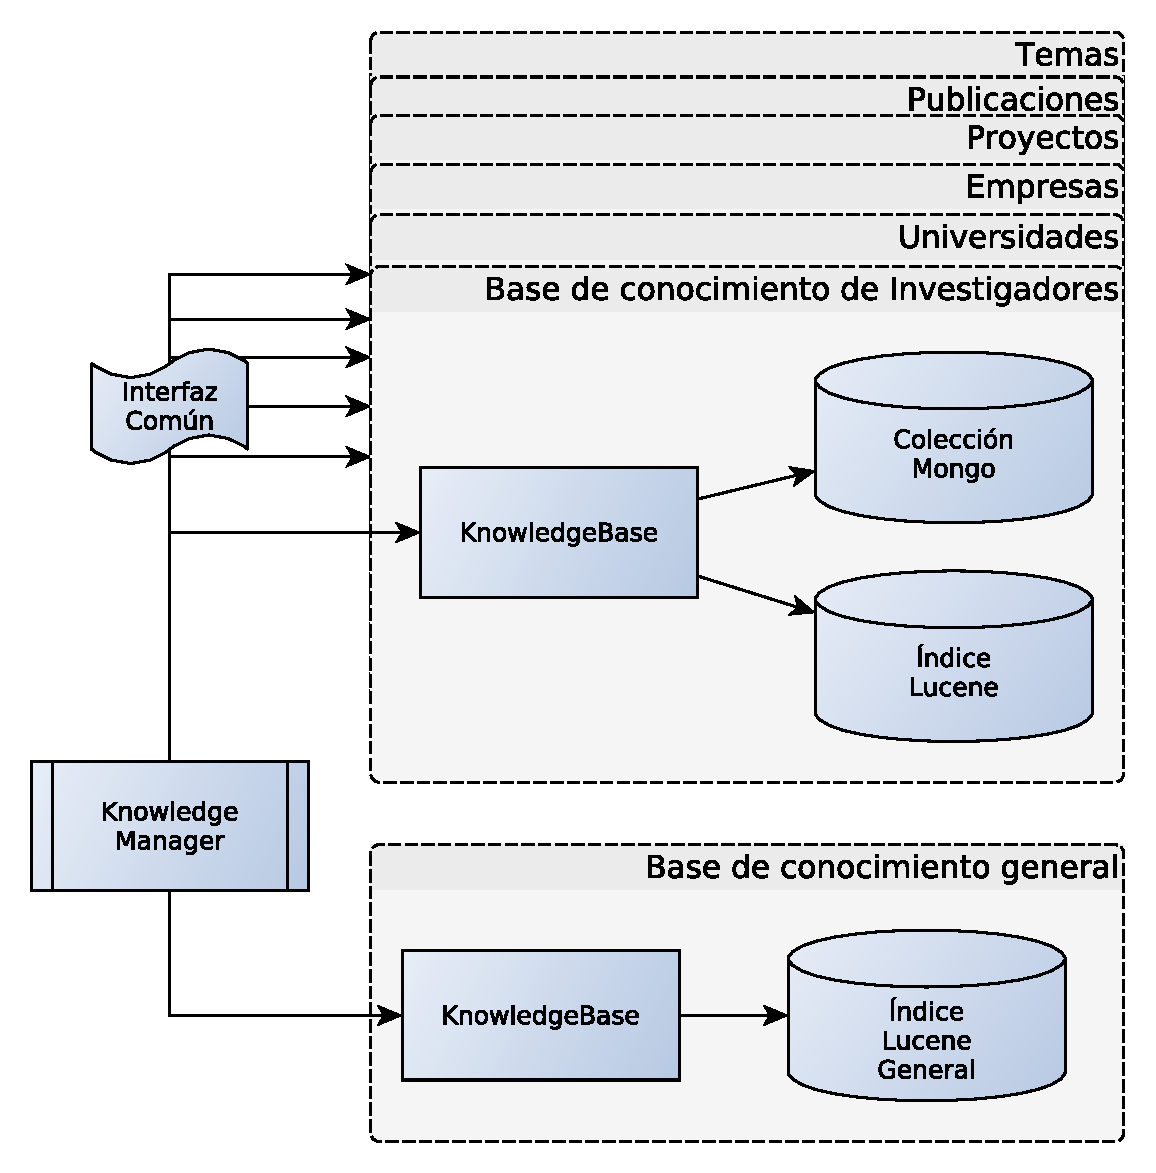
\includegraphics[scale=0.5]{graficos/KnowledgeManager}
  \caption{Base de Conocimiento de grafo de TICs}
  \label{fig:KnowledgeManager}
\end{figure}

\bigskip
\subsection{Dominio de datos}
\subsection{Modelo}
